%\documentclass[landscape,a0b,final,a4resizeable]{a0poster}
\documentclass[landscape,a0b,final]{a0poster}
%\documentclass[portrait,a0b,final,a4resizeable]{a0poster}
%\documentclass[portrait,a0b,final]{a0poster}
%%% Option "a4resizeable" makes it possible ot resize the
%   poster by the command: psresize -pa4 poster.ps poster-a4.ps
%   For final printing, please remove option "a4resizeable" !!

\usepackage{epsfig}
\usepackage{multicol}
\usepackage{cite}
\usepackage[font=footnotesize]{subfig}
\usepackage{float}
\usepackage{setspace}
\usepackage{wrapfig}
\usepackage{graphicx}
\usepackage{amsmath, amssymb, bm}
\DeclareMathOperator*{\argmin}{arg\,min}
\onehalfspacing
\usepackage{mathtools}
\usepackage{pstricks,pst-grad}
%%%%%%%%%%%%%%%%%%%%%%%%%%%%%%%%%%%%%%%%%%%
% Definition of some variables and colors
%\renewcommand{\rho}{\varrho}
%\renewcommand{\phi}{\varphi}
\setlength{\columnsep}{.5cm}
\setlength{\columnseprule}{2mm}
\setlength{\parindent}{0.0cm}

\usepackage{titlesec}

\titlespacing*{\section}
{0pt}{1ex}{1ex}



%%%%%%%%%%%%%%%%%%%%%%%%%%%%%%%%%%%%%%%%%%%%%%%%%%%%
%%%               Background                     %%%
%%%%%%%%%%%%%%%%%%%%%%%%%%%%%%%%%%%%%%%%%%%%%%%%%%%%

\newcommand{\background}[3]{
  \newrgbcolor{cgradbegin}{#1}
  \newrgbcolor{cgradend}{#2}
  \psframe[fillstyle=gradient,gradend=cgradend,
  gradbegin=cgradbegin,gradmidpoint=#3](0.,0.)(1.\textwidth,-1.\textheight)
}



%%%%%%%%%%%%%%%%%%%%%%%%%%%%%%%%%%%%%%%%%%%%%%%%%%%%
%%%                Poster                        %%%
%%%%%%%%%%%%%%%%%%%%%%%%%%%%%%%%%%%%%%%%%%%%%%%%%%%%

\newenvironment{poster}{
  \begin{center}
  \begin{minipage}[c]{0.98\textwidth}
}{
  \end{minipage}
  \end{center}
}



%%%%%%%%%%%%%%%%%%%%%%%%%%%%%%%%%%%%%%%%%%%%%%%%%%%%
%%%                pcolumn                       %%%
%%%%%%%%%%%%%%%%%%%%%%%%%%%%%%%%%%%%%%%%%%%%%%%%%%%%

\newenvironment{pcolumn}[1]{
  \begin{minipage}{#1\textwidth}
  \begin{center}
}{
  \end{center}
  \end{minipage}
}



%%%%%%%%%%%%%%%%%%%%%%%%%%%%%%%%%%%%%%%%%%%%%%%%%%%%
%%%                pbox                          %%%
%%%%%%%%%%%%%%%%%%%%%%%%%%%%%%%%%%%%%%%%%%%%%%%%%%%%

\newrgbcolor{lcolor}{0. 0. 0.80}
\newrgbcolor{gcolor1}{1. 1. 1.}
\newrgbcolor{gcolor2}{.80 .80 1.}

\newcommand{\pbox}[4]{
\psshadowbox[#3]{
\begin{minipage}[t][#2][t]{#1}
#4
\end{minipage}
}}



%%%%%%%%%%%%%%%%%%%%%%%%%%%%%%%%%%%%%%%%%%%%%%%%%%%%
%%%                myfig                         %%%
%%%%%%%%%%%%%%%%%%%%%%%%%%%%%%%%%%%%%%%%%%%%%%%%%%%%
% \myfig - replacement for \figure
% necessary, since in multicol-environment
% \figure won't work

\newcommand{\myfig}[3][0]{
\begin{center}
  \vspace{1.5cm}
  \includegraphics[width=#3\hsize,angle=#1]{#2}
  \nobreak\medskip
\end{center}}



%%%%%%%%%%%%%%%%%%%%%%%%%%%%%%%%%%%%%%%%%%%%%%%%%%%%
%%%                mycaption                     %%%
%%%%%%%%%%%%%%%%%%%%%%%%%%%%%%%%%%%%%%%%%%%%%%%%%%%%
% \mycaption - replacement for \caption
% necessary, since in multicol-environment \figure and
% therefore \caption won't work

%\newcounter{figure}
\setcounter{figure}{1}
\newcommand{\mycaption}[1]{
  \vspace{0.5cm}
  \begin{quote}
    {{\sc Figure} \arabic{figure}: #1}
  \end{quote}
  \vspace{1cm}
  \stepcounter{figure}
}



%%%%%%%%%%%%%%%%%%%%%%%%%%%%%%%%%%%%%%%%%%%%%%%%%%%%%%%%%%%%%%%%%%%%%%
%%% Begin of Document
%%%%%%%%%%%%%%%%%%%%%%%%%%%%%%%%%%%%%%%%%%%%%%%%%%%%%%%%%%%%%%%%%%%%%%

\begin{document}

\background{1. 1. 1.}{1. 1. 1.}{0.5}


\newrgbcolor{lightblue}{0. 0. 0.80}
\newrgbcolor{white}{1. 1. 1.}
\newrgbcolor{whiteblue}{.80 .80 1.}


\begin{poster}

%%%%%%%%%%%%%%%%%%%%%
%%% Header
%%%%%%%%%%%%%%%%%%%%%
\begin{center}
\begin{pcolumn}{1}

\pbox{0.97\textwidth}{}{linewidth=2mm,framearc=0.3,linecolor=lightblue,fillstyle=gradient,gradangle=0,gradbegin=white,gradend=whiteblue,gradmidpoint=1.0,framesep=1em}{

%%% Unisiegel
\begin{minipage}[c][9cm][c]{0.1\textwidth}
  \begin{center}
      %
\includegraphics[width=7cm,angle=0]{figs/k2.pdf}
  \end{center}
\end{minipage}
%%% Titel
\begin{minipage}[c][9cm][c]{0.78\textwidth}
  \begin{center}
      {\sc \veryHuge \textbf{A PSF photometry tool for NASA's Kepler,} $\bm{\mathcal{K}\mathit{2}}$\textbf{, and TESS missions}}\\[7mm]
      {\Large \textbf{Jos\'e Vin\'icius de Miranda Cardoso}$^{1, 2}$, \textbf{Geert Barentsen}$^{1, 2}$,
       \textbf{Benjamin T. Montet}$^{3, \bm{\star}}$, \textbf{Ann Marie Cody}$^{1, 2}$,}\\
      {\Large
       \textbf{Christina Hedges}$^{1, 2}$, \textbf{Michael Gully-Santiago}$^{1, 2}$, \textbf{Martin Still}$^{4}$, and
       \textbf{Thomas Barclay}$^{5}$}\\
      {\Large $^{1}$NASA Ames Research Center,
      $^{2}$Bay Area Environmental Research Institute,
      $^{3}$University of Chicago (NASA Sagan Fellow),
      $^{4}$NASA Headquarters,
      $^{5}$NASA Goddard}
  \end{center}
\end{minipage}
%%% GK-Logo
\begin{minipage}[c][9cm][c]{0.1\textwidth}
  \begin{center}
    %\includegraphics[width=7cm,angle=0]{}
  \end{center}
\end{minipage}

}
\end{pcolumn}
\end{center}

\vspace*{.5cm}

%%%%%%%%%%%%%%%%%%%%%
%%% Content
%%%%%%%%%%%%%%%%%%%%%
\begin{center}
\begin{pcolumn}{0.32}
\pbox{0.90\textwidth}{75cm}{linewidth=2mm,framearc=0.1,linecolor=lightblue,fillstyle=gradient,gradangle=0,gradbegin=white,gradend=white,gradmidpoint=1.0,framesep=1em}{

\begin{center}\pbox{0.8\textwidth}{}{linewidth=2mm,framearc=0.1,linecolor=lightblue,fillstyle=gradient,gradangle=0,gradbegin=white,gradend=whiteblue,gradmidpoint=1.0,framesep=1em}{\begin{center}\textbf{Introduction}\end{center}}\end{center}
\vspace{0.75cm}

\begin{itemize}
    \item NASA's Kepler and $\mathcal{K}\mathit{2}$ missions have been
        delivering high-precision time series data for a wide range of stellar types.
    \item However, both the official and community-developed
        pipelines~\cite{luger, vanderburg, aigrain} tend to focus on studying
        isolated stars using simple aperture photometry, which tends to perform
        sub-optimally in crowded fields and on faint stars. \cite{anderson, libralato1}.
    \item Although Point Spread Function (PSF) photometry methods are well
        known~\cite{anderson, libralato1}, open source tools to perform PSF
        photometry specifically on Kepler and $\mathcal{K}\mathit{2}$ data are scarce.
        To address this issue, we present an open source PSF photometry toolkit for
        Kepler and $\mathcal{K}\mathit{2}$, and extensible to TESS, as part of the
        $\mathcal{K}\mathit{2}$ Guest Observer Office data analysis toolkit, PyKE,
        \texttt{https://www.github.com/KeplerGO/pyke}.
    \item The code for this poster is available at: \\ \texttt{https://www.github.com/mirca/aas\_poster}.
\end{itemize}

\vspace{0.75cm}
\begin{center}\pbox{0.8\textwidth}{}{linewidth=2mm,framearc=0.1,linecolor=lightblue,fillstyle=gradient,gradangle=0,gradbegin=white,gradend=whiteblue,gradmidpoint=1.0,framesep=1em}{\begin{center}\textbf{Methods}\end{center}}\end{center}
\vspace{0.75cm}

    \begin{center}
        \textbf{Fitting multiple PSFs jointly}
    \end{center}

    Given an image with $n$ pixels and $m$ stars, we treat the pixel values $Y_i$ as
    independent \emph{non-identically} distributed Poisson random variables $\bm{Y} \triangleq \{Y_i\}_{i=1}^{n}$
    such that $\mathbb{E}\left[Y_i\right] = \sum_{j=1}^{m}\lambda_i(\bm{\Theta}_j)$,
    where $\lambda_i$ is the PSF model at the $i$-th pixel and $\bm{\Theta}_j$ is the
    vector of random variables which encode the flux and center of each star and the background.

    The likelihood function of the pixel values given the model parameters can then be written as
\begin{align}
   P\left(\bm{Y} = \bm{y} \Bigr| \left\{\bm{\Theta}_j\right\}_{j=1}^{m} = \left\{\bm{\theta}_j\right\}_{j=1}^{m}\right) = \exp\left({-\sum_{i=1}^{n}\sum_{j=1}^{m}\lambda_i(\bm{\theta}_j)}\right)\prod_{i=1}^{n}\dfrac{\left(\sum_{j=1}^{m}\lambda_i\left(\bm{\theta}_j\right)\right)^{y_i}}{y_i!}.
\end{align}

And the log likelihood function is
\begin{equation}
    \log  P\left(\bm{Y} = \bm{y} \Bigr| \left\{\bm{\Theta}_j\right\}_{j=1}^{m} = \left\{\bm{\theta}_j\right\}_{j=1}^{m}\right) = \sum_{i=1}^{n}\left(- \sum_{j=1}^{m}\lambda_i(\bm{\theta}_j) + y_i\log\sum_{j=1}^{m}\lambda_i(\bm{\theta}_j)\right).
\end{equation}

    Hence, the Maximum Likelihood Estimator can be formulated as the following optimization problem
\begin{align}
    \bm{\theta}^{*}(\bm{y}) = \argmin_{\bm{\theta} \in \Lambda} \sum_{i=1}^{n}\left(\sum_{j=1}^{m}\lambda_i(\bm{\theta}_j) - y_i\log\sum_{j=1}^{m}\lambda_i(\bm{\theta}_j)\right).
\end{align}
Note that it is often necessary to impose prior probability densities on the model parameters
    to aid the optimization.

\vspace{0.75cm}
    \begin{center}
        \textbf{Estimating uncertainties using the Cram\'er-Rao Lower Bound}
    \end{center}

Uncertainties on the fitted parameters are approximated using the Cram\'er-Rao Lower Bound. Mathematically,
        \begin{equation}
            cov(\bm{\theta}^{*}(\bm{Y})) = \left(\mathbb{E}_{\bm{\theta}}\left[\nabla_{\bm{\theta}}\log p(\bm{Y} | \bm{\theta})\left[\nabla_{\bm{\theta}}\log p(\bm{Y} | \bm{\theta}) \right]^{T}  \right]\right)^{-1}\Bigr|_{\substack{\bm{\theta}=\bm{\theta}^{*}(\bm{y})}}
        \end{equation}

}
\end{pcolumn}
\begin{pcolumn}{0.32}
\pbox{0.90\textwidth}{75cm}{linewidth=2mm,framearc=0.1,linecolor=lightblue,fillstyle=gradient,gradangle=0,gradbegin=white,gradend=white,gradmidpoint=1.0,framesep=1em}{


    \begin{center}
        \textbf{The Kepler Pixel Response Function Model}
        \begin{itemize}
            \item Kepler's pixel response function (PRF) has been shown to be nonsymmetric and spatially variant
                  accross the detector~\cite{bryson}.
            \item The PRF model used in PyKE is based on dithered data acquired during Kepler's comissioning phase~\cite{bryson}.
        \end{itemize}

        \includegraphics[width=15cm,angle=0]{figs/prf.eps}
        \includegraphics[width=15cm,angle=0]{figs/prf-contour.eps}

    \end{center}
            Using the PyKE package in Python, the PSF model for a given detector position can be instantiated using the information
            contained in Kepler Target Pixel File (TPF) header:\\
        \texttt{>>> from pyke import KeplerTargetPixelFile}\\
        \texttt{>>> tpf = KeplerTargetPixelFile("PATH")}\\
        \texttt{>>> prf = tpf.get\_prf\_model()}

%%% Section
        \vspace{1.0cm}
\begin{center}\pbox{0.8\textwidth}{}{linewidth=2mm,framearc=0.1,linecolor=lightblue,fillstyle=gradient,gradangle=0,gradbegin=white,gradend=whiteblue,gradmidpoint=1.0,framesep=1em}{\begin{center}\textbf{Crowded K2 Clusters}\end{center}}\end{center}\vspace{1.25cm}

Having instantiated suitable PSF models for a set of stars, we can use PyKE to
fit the joint model to the data.  In the example shown here, we simultaneously
fit five stars in data from the crowded Lagoon Nebula cluster observed during
$\mathcal{K}\mathit{2}$ Campaign 9. For the 14th-magnitude star shown in the
center of the cutout below, we find that PSF photometry yields a lightcurve
that is $\approx$ 3 times more precise compared to aperture photometry.
\vspace{1.0cm}

    \includegraphics[width=16cm,angle=0]{figs/tpf_c9.eps}
    \includegraphics[width=16cm,angle=0]{figs/model_c9.eps}
    \includegraphics[width=16cm,angle=0]{figs/residuals_c9.eps}
    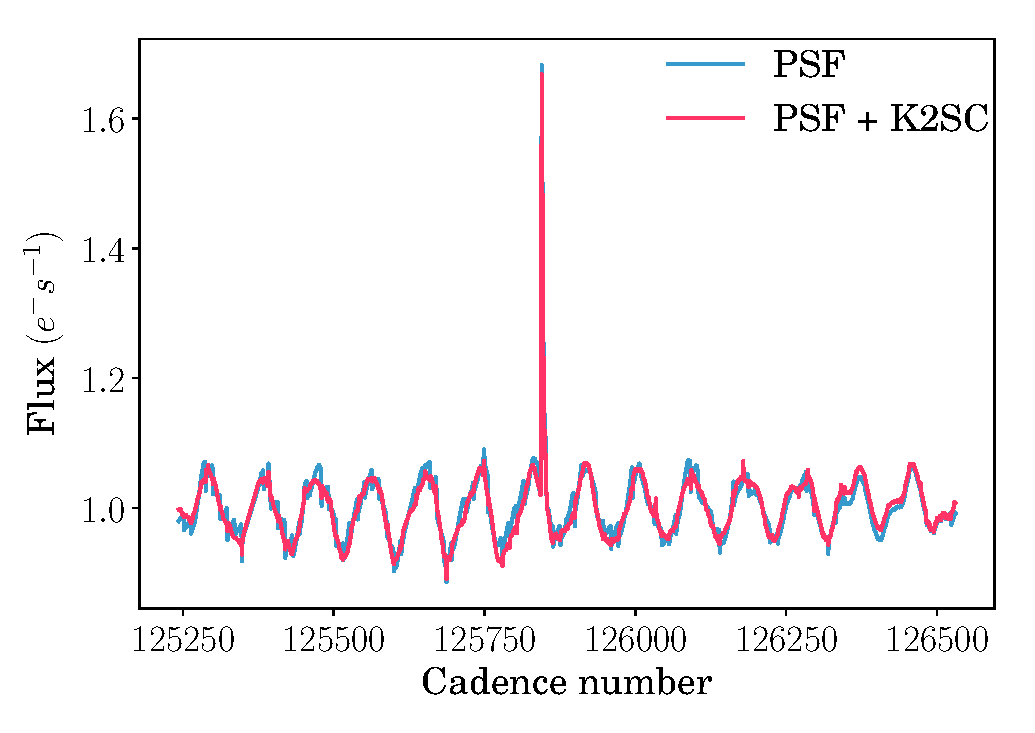
\includegraphics[width=17cm,angle=0]{figs/lc_c9.eps}

    \texttt{>>> from pyke.prf import SceneModel, PRFPhotometry}\\
    \texttt{>>> scene = SceneModel(prfs=5*[prf])} \\
    \texttt{>>> phot = PRFPhotometry(prior=prior, scene\_model=scene)} \\
    \texttt{>>> results = phot.fit(tpf.flux)} \\
}


\end{pcolumn}
\begin{pcolumn}{0.32}
\pbox{0.90\textwidth}{75cm}{linewidth=2mm,framearc=0.1,linecolor=lightblue,fillstyle=gradient,gradangle=0,gradbegin=white,gradend=white,gradmidpoint=1.0,framesep=1em}{

\begin{center}\pbox{0.8\textwidth}{}{linewidth=2mm,framearc=0.1,linecolor=lightblue,fillstyle=gradient,gradangle=0,gradbegin=white,gradend=whiteblue,gradmidpoint=1.0,framesep=1em}{\begin{center}\textbf{Kepler Faint Stars}\end{center}}\end{center}
\vspace{.5cm}

In addition to being necessary in crowded fields, we find that PSF photometry
also benefits the light curves of isolated faint stars. For example, star
\texttt{KIC 6444896} is known to contain a small planet, Kepler-1649b~\cite{isabel}.
Using PSF photometry, we recover the planet signal which is $\approx$ 1.67 times more precise
compared to the aperture photometry employed by the official Kepler pipeline.
Although the latter could be improved by tweaking the aperture mask of the source,
the fact that PSF photometry is not sensitive to the choice of an aperture mask is
a significant practical benefit.

    \begin{center}
\includegraphics[width=16cm,angle=0]{figs/tpf_kep.eps}
\includegraphics[width=16cm,angle=0]{figs/model_kep.eps}
\includegraphics[width=16cm,angle=0]{figs/residuals_kep.eps}
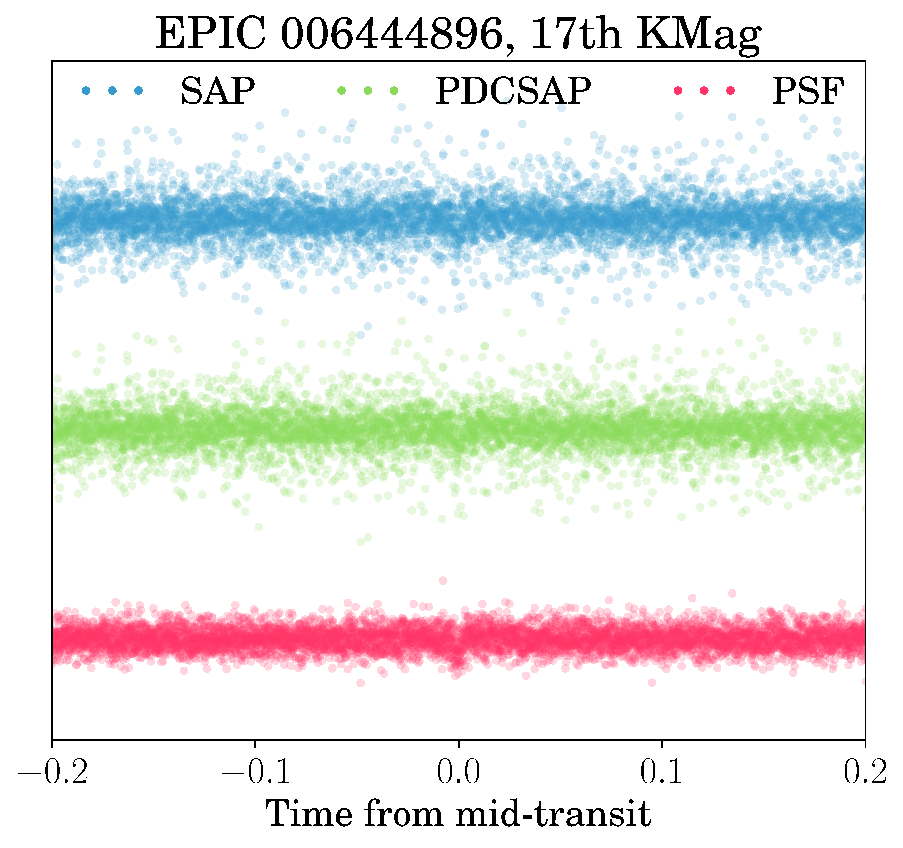
\includegraphics[width=16cm,angle=0]{figs/faint.eps}
    \end{center}

\begin{center}\pbox{0.8\textwidth}{}{linewidth=2mm,framearc=0.1,linecolor=lightblue,fillstyle=gradient,gradangle=0,gradbegin=white,gradend=whiteblue,gradmidpoint=1.0,framesep=1em}{\begin{center}\textbf{Conclusions}\end{center}}\end{center}
\vspace{.5cm}

    \begin{itemize}
        \item We have presented an open-source tool to perform PSF photometry on Kepler and $\mathcal{K}\mathit{2}$ data.
        \item For crowded clusters and faint stars, we find that PSF photometry can outperform aperture photometry.
        \item In future work, we intend to infer the PSF model from nearby stars to improve the accuracy of the fit.
            We will also study the performance as a function of stellar brightness and crowding.
    \end{itemize}

%%% References
\bibliographystyle{unsrt}
    {\small \bibliography{poster.bib}}

}
\end{pcolumn}
\end{center}

\end{poster}

\end{document}

